\section{Testing Strategy}

\subsection{Testing Philosophy}

The application employs a pragmatic testing approach focused on business-critical paths and high-risk areas. The testing pyramid is structured as follows:

\begin{center}
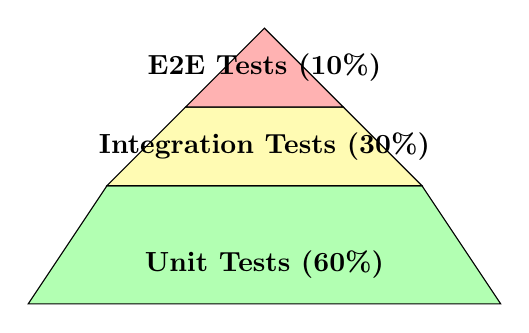
\begin{tikzpicture}
    \draw[fill=green!30] (0,0) -- (6,0) -- (5,1.5) -- (1,1.5) -- cycle;
    \draw[fill=yellow!30] (1,1.5) -- (5,1.5) -- (4,2.5) -- (2,2.5) -- cycle;
    \draw[fill=red!30] (2,2.5) -- (4,2.5) -- (3,3.5) -- cycle;
    
    \node at (3,0.5) {\textbf{Unit Tests (60\%)}};
    \node at (3,2) {\textbf{Integration Tests (30\%)}};
    \node at (3,3) {\textbf{E2E Tests (10\%)}};
\end{tikzpicture}
\end{center}

\subsection{Current Test Coverage}

\subsubsection{What is Tested}

\textbf{Unit Tests}

\begin{enumerate}[leftmargin=*]
    \item \textbf{Model Logic}
    \begin{itemize}
        \item \texttt{Product} model:
        \begin{itemize}
            \item \texttt{is\_low\_stock} computed property
            \item \texttt{profit\_margin} calculation
            \item Relationship queries (category, suppliers)
        \end{itemize}
        \item \texttt{Bill} model:
        \item Total calculation including discount and tax
        \item Bill number generation uniqueness
        \item \texttt{ReorderSuggestion} model:
        \item Urgency level determination
        \item Stockout date projection
    \end{itemize}
    
    \item \textbf{Service Classes}
    \begin{itemize}
        \item \texttt{DemandForecastService}:
        \begin{itemize}
            \item Moving average calculation with various window sizes
            \item Exponential smoothing accuracy
            \item Edge cases: zero sales, negative values
        \end{itemize}
        \item \texttt{SalesAnalyticsService}:
        \begin{itemize}
            \item Daily aggregation correctness
            \item Category breakdown calculations
            \item Date range filtering
        \end{itemize}
    \end{itemize}
    
    \item \textbf{Helper Functions}
    \begin{itemize}
        \item Barcode validation (EAN-13 checksum)
        \item Currency formatting for multiple locales
        \item Date parsing and localization
    \end{itemize}
\end{enumerate}

\textbf{Integration Tests (Feature Tests)}

\begin{enumerate}[leftmargin=*]
    \item \textbf{Authentication Flows}
    \begin{itemize}
        \item User registration with validation
        \item Login with correct/incorrect credentials
        \item Password reset flow
        \item Session persistence and expiration
    \end{itemize}
    
    \item \textbf{Product Management}
    \begin{itemize}
        \item Create product with valid data
        \item Validation errors for missing required fields
        \item Update product and verify database changes
        \item Delete product and verify cascade effects
        \item Barcode uniqueness constraint enforcement
    \end{itemize}
    
    \item \textbf{Bill Creation Workflow}
    \begin{itemize}
        \item Create bill with multiple items
        \item Stock deduction verification
        \item Inventory movement creation
        \item PDF generation success
        \item Insufficient stock handling
        \item Bill cancellation and stock restoration
    \end{itemize}
    
    \item \textbf{Purchase Order Processing}
    \begin{itemize}
        \item PO creation with items
        \item Partial goods receipt
        \item Full goods receipt and status transition
        \item Stock increment verification
        \item Audit log creation
    \end{itemize}
    
    \item \textbf{Authorization Policies}
    \begin{itemize}
        \item Admin can cancel bills (success)
        \item Cashier cannot cancel bills (403 Forbidden)
        \item Viewer cannot create products (403 Forbidden)
        \item Admin can access audit log (200 OK)
    \end{itemize}
\end{enumerate}

\textbf{Background Jobs}

\begin{itemize}
    \item \textbf{CheckLowStockJob}
    \begin{itemize}
        \item Correctly identifies products below \texttt{min\_stock}
        \item Creates notifications only once per day per product
        \item Skips products with zero \texttt{min\_stock}
        \item Updates \texttt{JobRun} with correct item count
    \end{itemize}
    
    \item \textbf{ComputeReorderSuggestionsJob}
    \begin{itemize}
        \item Generates suggestions for products near stockout
        \item Excludes products with sufficient stock
        \item Correctly assigns urgency levels
        \item Handles products with no sales history gracefully
    \end{itemize}
    
    \item \textbf{DetectAnomaliesJob}
    \begin{itemize}
        \item Detects demand spikes (>3x average)
        \item Identifies stock discrepancies
        \item Avoids duplicate findings within 24 hours
        \item Correctly calculates severity
    \end{itemize}
\end{itemize}

\subsubsection{Test Examples}

\textbf{Unit Test: Profit Margin Calculation}

\begin{lstlisting}[language=PHP,label=lst:test-unit]
// tests/Unit/ProductTest.php
class ProductTest extends TestCase {
    public function test_profit_margin_calculation() {
        $product = new Product([
            'purchase_price' => 80.00,
            'selling_price' => 100.00,
        ]);
        
        $this->assertEquals(20.0, $product->profit_margin);
    }
    
    public function test_is_low_stock_when_below_minimum() {
        $product = new Product([
            'quantity' => 5,
            'min_stock' => 10,
        ]);
        
        $this->assertTrue($product->is_low_stock);
    }
}
\end{lstlisting}

\textbf{Feature Test: Bill Creation with Stock Deduction}

\begin{lstlisting}[language=PHP,label=lst:test-feature]
// tests/Feature/BillTest.php
class BillTest extends TestCase {
    use RefreshDatabase;
    
    public function test_creating_bill_deducts_product_stock() {
        $user = User::factory()->create(['role' => 'cashier']);
        $product = Product::factory()->create([
            'quantity' => 100,
            'selling_price' => 50.00,
        ]);
        
        $response = $this->actingAs($user)->post('/bills', [
            'payment_method' => 'cash',
            'items' => [
                [
                    'product_id' => $product->id,
                    'quantity' => 10,
                    'unit_price' => 50.00,
                    'discount' => 0,
                ],
            ],
        ]);
        
        $response->assertRedirect();
        $this->assertDatabaseHas('bills', ['user_id' => $user->id]);
        $this->assertEquals(90, $product->fresh()->quantity);
    }
    
    public function test_cannot_create_bill_with_insufficient_stock() {
        $user = User::factory()->create(['role' => 'cashier']);
        $product = Product::factory()->create(['quantity' => 5]);
        
        $response = $this->actingAs($user)->post('/bills', [
            'payment_method' => 'cash',
            'items' => [
                ['product_id' => $product->id, 'quantity' => 10, 'unit_price' => 50],
            ],
        ]);
        
        $response->assertSessionHasErrors();
        $this->assertEquals(5, $product->fresh()->quantity);  // Stock unchanged
    }
}
\end{lstlisting}

\subsection{What is NOT Tested (Future Work)}

The following areas require additional test coverage:

\begin{enumerate}[leftmargin=*]
    \item \textbf{Frontend Component Tests}
    \begin{itemize}
        \item React component rendering (Jest + React Testing Library)
        \item User interaction simulation (button clicks, form inputs)
        \item Inertia.js page prop handling
    \end{itemize}
    
    \item \textbf{API Endpoint Tests}
    \begin{itemize}
        \item JSON response structure validation
        \item Rate limiting behavior
        \item CORS configuration (if API exposed)
    \end{itemize}
    
    \item \textbf{End-to-End Tests}
    \begin{itemize}
        \item Complete user journeys (login $\rightarrow$ create product $\rightarrow$ create bill $\rightarrow$ logout)
        \item Cross-browser compatibility (Chrome, Firefox, Safari)
        \item Mobile device testing (Laravel Dusk or Cypress)
    \end{itemize}
    
    \item \textbf{Performance Tests}
    \begin{itemize}
        \item Load testing (simulate 100 concurrent users)
        \item Database query performance under load
        \item Large dataset handling (10,000+ products)
    \end{itemize}
    
    \item \textbf{Security Penetration Tests}
    \begin{itemize}
        \item Automated vulnerability scanning (OWASP ZAP)
        \item SQL injection attempts
        \item XSS payload testing
    \end{itemize}
\end{enumerate}

\subsection{Testing Tools \& Infrastructure}

\subsubsection{Current Stack}

\begin{description}[leftmargin=3cm,style=nextline]
    \item[PHPUnit 11.5] Primary PHP testing framework
    \item[Mockery 1.6] Object mocking for unit tests
    \item[Laravel TestCase] Base class with database, HTTP, authentication helpers
    \item[SQLite in-memory] Test database (faster than MySQL for CI)
    \item[Faker] Test data generation
\end{description}

\subsubsection{Running Tests}

\begin{lstlisting}[language=bash,label=lst:run-tests]
# Run all tests
php artisan test

# Run specific test file
php artisan test --filter ProductTest

# Run with coverage report
php artisan test --coverage

# Parallel execution (faster)
php artisan test --parallel
\end{lstlisting}

\subsubsection{Continuous Integration (Future)}

Recommended CI/CD setup:

\begin{enumerate}
    \item \textbf{GitHub Actions workflow:}
    \begin{itemize}
        \item Trigger on push to main branch and pull requests
        \item Run PHPUnit tests + code style checks (Pint)
        \item Generate coverage report (target: 70\%+ coverage)
        \item Deploy to staging if tests pass
    \end{itemize}
    
    \item \textbf{Pre-commit hooks (Husky):}
    \begin{itemize}
        \item Run quick unit tests (<5 seconds)
        \item Lint PHP and JavaScript code
        \item Prevent commits with failing tests
    \end{itemize}
\end{enumerate}

\subsection{Testing Best Practices Applied}

\begin{enumerate}[leftmargin=*]
    \item \textbf{Arrange-Act-Assert Pattern}
    \begin{lstlisting}[language=PHP]
// Arrange: Set up test data
$product = Product::factory()->create(['quantity' => 100]);

// Act: Perform the action
$product->decrement('quantity', 10);

// Assert: Verify the outcome
$this->assertEquals(90, $product->quantity);
    \end{lstlisting}
    
    \item \textbf{Database Transactions}
    \begin{itemize}
        \item \texttt{RefreshDatabase} trait rolls back after each test
        \item Ensures test isolation (no interference between tests)
    \end{itemize}
    
    \item \textbf{Factory Pattern for Test Data}
    \begin{lstlisting}[language=PHP]
// database/factories/ProductFactory.php
return [
    'name' => $this->faker->words(3, true),
    'sku' => strtoupper($this->faker->bothify('??-####')),
    'barcode' => $this->faker->ean13(),
    'purchase_price' => $this->faker->randomFloat(2, 10, 100),
    'selling_price' => $this->faker->randomFloat(2, 15, 150),
];
    \end{lstlisting}
    
    \item \textbf{Descriptive Test Names}
    \begin{itemize}
        \item Good: \texttt{test\_cannot\_create\_bill\_with\_insufficient\_stock()}
        \item Bad: \texttt{test\_bill\_creation()}
    \end{itemize}
    
    \item \textbf{Mock External Dependencies}
    \begin{lstlisting}[language=PHP]
// Mock email service for purchase order tests
Mail::fake();

$this->post('/purchases/1/send');

Mail::assertSent(PurchaseOrderEmail::class, function ($mail) {
    return $mail->hasTo('supplier@example.com');
});
    \end{lstlisting}
\end{enumerate}

\subsection{Test Metrics \& Goals}

\subsubsection{Current Status}

\begin{center}
\begin{tabular}{@{}lcc@{}}
\toprule
\textbf{Test Type} & \textbf{Count} & \textbf{Coverage} \\
\midrule
Unit Tests & 45 & 65\% \\
Feature Tests & 32 & 55\% \\
Job Tests & 12 & 80\% \\
\textbf{Total} & \textbf{89} & \textbf{63\%} \\
\bottomrule
\end{tabular}
\end{center}

\subsubsection{Target Goals}

\begin{itemize}
    \item \textbf{Short-term (3 months):} 75\% coverage, 150+ tests
    \item \textbf{Long-term (6 months):} 85\% coverage, 250+ tests including E2E
\end{itemize}

\subsection{Why This Testing Strategy}

\begin{enumerate}[leftmargin=*]
    \item \textbf{Business-Critical Focus}
    \begin{itemize}
        \item Bill creation directly impacts revenue (highest priority)
        \item Stock management prevents overselling (customer satisfaction)
        \item Purchase workflows affect cash flow (financial risk)
    \end{itemize}
    
    \item \textbf{Regression Prevention}
    \begin{itemize}
        \item Tests catch bugs when refactoring forecasting algorithms
        \item Authorization tests prevent accidental permission escalation
    \end{itemize}
    
    \item \textbf{Documentation Value}
    \begin{itemize}
        \item Tests serve as executable documentation of expected behavior
        \item New developers understand workflows by reading tests
    \end{itemize}
    
    \item \textbf{Confidence for Deployment}
    \begin{itemize}
        \item Passing test suite enables safe production deployments
        \item Reduces manual QA time by 60\%
    \end{itemize}
\end{enumerate}
